%Notes to myself:
%ABS:
%   http://abs-models.org/documentation/manual/#sec:algebraic-data-types
%   http://delivery.acm.org/10.1145/3130000/3122848/a76-boer.pdf?ip=130.238.252.224&id=3122848&acc=ACTIVE%20SERVICE&key=74F7687761D7AE37%2EDA50417A8F734F4C%2E4D4702B0C3E38B35%2E4D4702B0C3E38B35&CFID=1012165178&CFTOKEN=22086748&__acm__=1512138297_7db1453bc51abbd04fa38d02cff9f460 Page >= 11
%
%
%
%

\documentclass[10pt]{report}

\usepackage[utf8]{inputenc}
\usepackage{float}
%\setlength{\parindent}{0pt} % no auto indent

% CLICKABLE LINKS IN TOC,CITE,REF, ETC.
\usepackage[hidelinks]{hyperref}

% TABLES
\usepackage{tabularx,booktabs,multirow,bigdelim} % for big parenthesis on side of table
\usepackage[table]{xcolor}

% GRAPHICS
\usepackage{graphicx}
\graphicspath{{images/}}
\usepackage{pgfplots}

% BIBLIOGRAPHY
%\usepackage[bibstyle=nature, citestyle=numeric-comp]{biblatex}
%\usepackage{natbib}
%\bibliographystyle{plain} % plain
\bibliography{references}

% APPENDICES
\usepackage[toc,page]{appendix}

% CHAPTER STYLE
\usepackage{titlesec}
\titleformat{\chapter}{\normalfont\huge}{\thechapter.}{20pt}{\huge\bf}

% TIKZ
\usepackage{tikz}
\usepackage{pgf}
\usetikzlibrary{trees}
\usetikzlibrary{shadows,positioning}

% COLORS
\usepackage{color}
\definecolor{eclipseBlue}{RGB}{42,0.0,255}
\definecolor{eclipseGreen}{RGB}{63,127,95}
\definecolor{eclipsePurple}{RGB}{127,0,85}
\definecolor{codeListingBackground}{gray}{0.95}

% CODE LISTINGS
\usepackage{listings}
\usepackage{caption,subcaption}
\setcounter{tocdepth}{5}
\setcounter{secnumdepth}{3}
\setlength{\parindent}{0pt}
\hangafter=0
\usepackage[parfill]{parskip}
%% Define Language
\lstdefinelanguage{Encore}
{
  morekeywords={
  active,
  case,catch,chain,class,data,
  def,do,
  eos,else,end,exception,
  finally,for,fun,
  get,getNext,
  if,import,in,
  let,linear,
  match,module,new,
  print,println,
  qualified,
  return,require,
  shared,stream,
  then,this,throw,trait,try,typedef,
  unless,unsafe,
  val,var,
  when,where,while,with,
  yield
  },
  sensitive=true, % keywords are not case-sensitive
  morecomment=[l]{--}, % l is for line comment
  morestring=[b]" % defines that strings are enclosed in double quotes
}
\lstdefinelanguage{C}
{
  morekeywords={
  int64_t, void, list_t, if, else, NULL, 
  sealed, trait, =>
  },
  sensitive=true, % keywords are not case-sensitive
  morecomment=[l]{--}, % l is for line comment
  morestring=[b]" % defines that strings are enclosed in double quotes
}

\lstdefinelanguage{Scala}
{
  morekeywords={
  match, case, object, class, extends,
  sealed, trait, =>
  },
  sensitive=true, % keywords are not case-sensitive
  morecomment=[l]{--}, % l is for line comment
  morestring=[b]" % defines that strings are enclosed in double quotes
}

%\lstset{numbers=left,xleftmargin=2em,frame=single,framexleftmargin=1.5em}

\lstset{
%  language={Encore},
  basicstyle=\footnotesize\ttfamily, % Global Code Style
  backgroundcolor=,%\color{codeListingBackground},
  captionpos=b, % Position of the Caption (t for top, b for bottom)
  extendedchars=true, % Allows 256 instead of 128 ASCII characters
  tabsize=1, % number of spaces indented when discovering a tab
  columns=fixed, % make all characters equal width
  keepspaces=true, % does not ignore spaces to fit width, convert tabs to spaces
  showstringspaces=false, % lets spaces in strings appear as real spaces
  breaklines=true, % wrap lines if they don't fit
  frame=none, % e.g. none/tbrl/single/lines. tbrl = draw a frame at the top, right, left and bottom of the listing.
  xleftmargin=2ex,
  framexleftmargin=0pt,
  framexrightmargin=0pt,
  framextopmargin=0pt,
  framexbottommargin=0pt,
  frameround=ffff, % make the frame round at all four corners
  framesep=0pt, % quarter circle size of the round corners
  numbers=left, %left, % show line numbers at the left
  numberstyle=\color{eclipseBlue}\tiny\ttfamily, % style of the line numbers
  numbersep=3pt, % distance between numbers and code
  commentstyle=\color{eclipseGreen}, % style of comments
  keywordstyle=\bf, % style of keywords \color{eclipsePurple}
  stringstyle=, % style of strings \color{eclipseBlue}
  showlines=true,
  linewidth=20cm,
}

\lstdefinestyle{encattachment} {
  language=Encore,
  frame=none,
  captionpos=t,
  numbers=none,
  frame=tbrl,
  framexleftmargin=2pt,
  framexrightmargin=2pt,
  framextopmargin=2pt,
  framexbottommargin=2pt,
}

\newcommand{\KIKO}[1]{\textcolor{red}{\textbf{[Kiko: #1]}}}

% CUSTOM COMMANDS
\def\code#1{\texttt{#1}} % Code-esque text
\def\todo#1{\textcolor{blue}{\{TODO: #1\}}}
\def\name#1{\textsc{#1}} % Proper nouns, names, logos, names of programming languages

\title{
    {Algebraic data types in Encore:}\\
    {reconciling objection-oriented and functional programming}\\
    {Uppsala University}
}

\author{Micael Loberg}
\date{\today}

\begin{document}
\pagenumbering{roman}

\maketitle

\newpage\newpage
%\vspace*{\fill}
{\centering \textit{This page intentionally left blank}\par}
\vspace{\fill}


\chapter*{Abstract}
\par{Encore is an object-oriented programming language with a focus on implementing concurrent and parallel systems. Unlike traditional object-oriented programming languages, each object in Encore has its own thread of control. Encore also has passive objects which lack their own thread of control, these are mainly used to create data structures such as lists or trees and are used inside of active objects. This thesis presents Algebraic Data Types (ADTs) as a complement to passive classes, and explores how this construct that is normally found in functional languages can be a useful addition to an object-oriented language such as Encore. The implementation takes advantage of the fact that the Encore compiler has a desugaring phase where the ADT syntax is transformed to traits and passive classes. This paper discusses the design of the syntax and the behaviour of Algebraic Data Types with concurrent and parallel systems in mind. Optimizations have also been made as to how pattern matching is done when used together with Algebraic Data Types.}

\newpage\newpage
%\vspace*{\fill}
{\centering \textit{This page intentionally left blank}\par}
\vspace{\fill}


\tableofcontents

%\KIKO{Maybe an introduction similar to the style of Gustav's thesis, where
%he gives a brief intro and the project goal. Right after that, the background}

%%%%%%%%%%%%%%%%%%%%%%%%%%%%%%%%%%%%%%%%%%%%%
%
\chapter{Background}
%
%%%%%%%%%%%%%%%%%%%%%%%%%%%%%%%%%%%%%%%%%%%%%
\pagenumbering{arabic}
\setcounter{page}{1}

%%%%%%%%%%%%%%%%%%%%%%%%%%%%%%%%%%%%%%%%%%%%%
%
\label{ch:background}
%
%%%%%%%%%%%%%%%%%%%%%%%%%%%%%%%%%%%%%%%%%%%%%

\section{Encore}
\par{Encore is an object-oriented programming language that is being developed at Uppsala University\cite{Encore}. It has a focus on implementing concurrent and parallel systems and it is using the Actor model. Encore has active objects that have their own thread of control and they can communicate with each other through message passing. Encore also has passive objects; these lack their own thread of control and behave like objects in more traditional object-oriented programming languages such as C++ or Java. Passive objects are mainly used to create data structures such as lists or trees and are used inside of active objects. Instead of the standard class-based inheritance, Encore uses traits.  A trait is a composable unit of behaviour that provides a set of methods and requires a set of fields and methods from any class that wishes to include it.} %TODO: write moar stuffs!
\section{Algebraic Data Types}
\par{Functional languages use Algebraic data types (ADTs) to describe composite data. Data structures can in type theory be described in terms of products, sums and recursive types. This leads to an algebra for describing data structures (hence Algebraic Data Types). Such data types are common in functional languages, such as ML or Haskell.}

\par{Robert Harper describes \textbf{Products} of types in the book \textit{'Practical Foundations for Programming Languages'} as the following:}

\par{\textit{"The binary \textbf{product} of two types consists of ordered pairs of values, one from each type in the order specified. The associated eliminatory forms are projections, which select the first and second component of a pair. The nullary product, or unit, type consists solely of the unique “null tuple” of no values, and has no associated eliminatory form."}}
\par{An example of a \textbf{product type} is a tuple consisting of a \code{bool} and an \code{int}, \code{(bool, int)}.}
\par{\textbf{Sums types} can be seen as the choice of two or more variants of a data structure. Some type \code{Foo} could be defined as the choice between an \code{int} or a \code{bool}. In Haskell this could be defined as \code{data Foo = bool | int}.}

%TODO: Make listing work
\par{An example of a data structure that is both a sum and product type can be seen in listing~\ref{lst:e4c_syntax}. It is an example of a polymorphic binary tree implemented using ADTs. Here \code{Tree} is the name of the type constructor and \code{Nil} and \code{Branch} are data constructors that are used to create new instances of type \code{Tree} and \code{t} is a type variable. The type \code{Tree} is also recursive as it is defined in terms of itself.}


\begin{lstlisting}[language=Haskell,caption={Binary tree definition in Haskell},label={lst:e4c_syntax}]
data Tree t = Nil
            | Branch t (Tree t) (Tree t)
\end{lstlisting}
%\subsection{ADTs In Functional Languages}% (this section has more become something like 'ADTs vs Classes' :/ )
%\par{In the C programming language sum types can be created using unions, product types can be created with structs and types can be recursive by also holding a pointer to its own type. In the previous chapter we saw how ADTs can be used to create both sum and product types, as well as recursive types. Most functional languages does not all of these other constructs, so the primary method of defining composite data is with Algebraic Data Types}

%\KIKO{I found this paper, which seems relevant: https://dl.acm.org/citation.cfm?doid=1094811.1094814, "Generalized algebraic data types and object-oriented programming"}
%\KIKO{I find this introduction a bit abrupt. Maybe ADTs started in the functional setting to solve a problem and you can continue from there.}
%In most functional languages there are no objects, so the primary method of defining composite data is with Algebraic Data Types.

%\KIKO{What do you mean? This first sentence is not clear.}
%Though ADTs is in no way equivalent with classes. Some of the major differences is mutability. Instance variables in a class is generally mutable while values in an ADT is not. Another distinction is that Algebraic Data Types allow for both sums and products while classes only allows for products.
%\KIKO{Maybe I am mistaken but Animal<t> has subclasses Cat<t> and Dog<t>. Can a polymorphic class be considered sum type? I am not saying that it is, I am asking.}

%ADTs also expose their insides to the world in a way that classes do not. This allows the programmer to perform pattern matching on the structure of an Algebraic Data Type. Pattern matching on the structure of types is also a feature that is mostly found in Functional languages and is critical to work with ADTs an effective manner.
\subsection{ADTs In Imperative/OO Languages}
\par{While Algebraic Data Types are mostly found in functional languages, there are examples of imperative languages that feature them. Here we will study two such languages so that we can get some insight as to what might be a good design for ADTs in Encore.}
\subsubsection{Scala}
\par{Scala is a multi-paradigm, general purpose language that features ADTs.}
\par{A binary tree in Scala could have the following definition:}

\begin{lstlisting}[language=Scala,caption={ADT definition in Scala},label={lst:e4c_syntax}]
sealed trait Tree[+T]
case object Nil extends Tree[Nothing]
case class Branch[T](value:T, left:Tree[T], right:Tree[T]) extends Tree[T]
\end{lstlisting}
\par{Noteworthy here is that the ADT is defined in terms of a trait and classes extending the trait. In Scala a sealed trait is a special kind of trait that can only be extended in the same file as it is defined. A case class is mostly a normal class with a few differences, such as it being immutable\cite{ScalaCase}. Case classes can also be used in pattern matching:}
\begin{lstlisting}[language=Scala,caption={Pattern matching on an ADT in Scala},label=scala-match]
tree match {
    case Branch(value, left, right) => Foo()
    case Nil()  => Bar()
}
\end{lstlisting}
\par{One can easily see the similarities of this implementation and the one in listing \ref{scala-match}. Here \code{Tree} is a type constructor, \code{Nil} and \code{Branch} are data constructors.}
\par{Scala uses a scheme of traits and classes to encode its algebraic data types. Also, it allows for case classes to be used in destructured pattern matching. This allows for programming patterns normally found only in functional languages.}
\subsubsection{ABS}%TODO: Bababa
\par{The Abstract Behavioral Specification language\cite{ABS} (ABS) is another language that features ADTs. It is a language that is interesting to look at because just like Encore it is an Object Oriented language that uses the Actor model as its concurrency model. When implementing ADTs in Encore, some design decisions had to be made and looking at another language that faced with the same design decisions gave some insight of what a good design could be. One such example is that of mutability. In ABS all values held by an ADT are immutable. The reasoning behind this is to make them safe to pass around between different actors and that it makes it easier to reason about the code\cite{ABSmut}}
\par{A linked list containing Integers can be defined as}
\begin{lstlisting}[language=encore,caption={Linked list in ABS}]
data List = Nil
          | Node(Int value, List tail);
\end{lstlisting}
\par{Names for constructors and their arguments can optionally be omitted, an example is the following implementation of the Bool datatype\}

% KIKO: I would recomment that listings have a \label as well, e.g.
\begin{lstlisting}[language=encore,caption={Actual definition of built-in type Bool},label=test-kiko]
data Bool = True | False;
\end{lstlisting}

\par{If data constructor arguments have names, like \code{head} and \code{tail} (Listing \ref{abs-list}) - it defines a function that, when passed a value expressed with the given constructor, returns the argument.  The name of an accessor function must be unique in the module it is defined in. It is an error to have multiple accessor functions with the same name, or to have a function definition with the same name as an accessor function.}

\begin{lstlisting}[language=encore,caption={Accessor funtion in ABS},label=abs-list]
data List = Nil
          | Node(Int head, List tail);
{
  List list = List(1, List(2, Nil));
  Int head = head(list); #Variable head is assigned the value 1
}
\end{lstlisting}

\chapter{Encoding ADTs in Encore}
\par{In Encore it is currently possible to emulate the behaviour of ADTs using a scheme of traits and classes.\cite{gustavL}. In this chapter we will give an example how this is done, and also discuss some of the problems inherent in using this scheme.}
\subsection{Encoding scheme}
\par{An implementation of a linked list in Encore could consist of the two classes \code{Node} and \code{Last}, both of which implement the trait \code{LinkedList}}
\par{Classes can implement extractor methods that exposes the internal structure of an object which can then be used in pattern matching. If the trait \code{LinkedList} requires the classes who implements the trait to also implement extractor methods, an object of type \code{LinkedList} can be used in pattern matching}

\begin{lstlisting}[language=encore,caption={trait LinkedList that requires classes to implement destructor methods}]
trait LinkedList[t]
  require def Node() : Maybe[(t, LinkedList)]
  require def Last() : Maybe[(t)]
end
\end{lstlisting}
\par{The class \code{Node} in listing \ref{encoding-scheme} will implement both of the extractor methods \code{Node()} and \code{Last()}. The method \code{Node()} will return an option type containing a tuple consisting of the internal objects to be exposed, in this case \code{value} and \code{next} while the method \code{Last()} will return \code{Nothing}}

\par{Similarly an object of type \code{Last} (listing \ref{encoding-scheme}) will also implement both extractor methods \code{Node()} and \code{Last()}. Though here the method \code{Node()} will return \code{Nothing} while \code{Last()} returns \code{Just(value).}}

\begin{lstlisting}[language=encore,caption={Implementation of Node and Last classes},label=encoding-scheme]
read class Node[t] : List[t](value, next)
  val value : t
  val next : List[t]

  def init(value : t, next : List[t]) : unit
    this.value = value
    this.next = next
  end

  def Last() : Maybe[t]
    Nothing
  end

  def Node() : Maybe[(t, List[t])]
    Just((this.value, this.next))
  end
end

read class Last[t] : List[t](value)
  val value : t

  def init(value : t) : unit
    this.value = value
  end

  def Last() : Maybe[t]
    Just(this.value)
  end

  def Node() : Maybe[(t, List[t])]
    Nothing
  end
end
\end{lstlisting}

\par{To make the classes \code{Node} and \code{Last} look more like branches of an ADT and hide the fact that they are classes, we also add constructor functions to create the objects for us.}

\begin{lstlisting}[language=encore,caption={Constructor functions for Node and Last}]
fun Node[t](value : t, next : List[t]) : List[t]
  new Node[t](value, next)
end

fun Last[t](value : t) : List[t]
  new Last[t](value)
end
\end{lstlisting}

\par{A LinkedList containing the values $[1, 2, 3]$ can now be created like this}
\begin{lstlisting}[language=encore,caption={Creation of list containing three elements}]
var list = Node(1, Node(2, Last(3)))
\end{lstlisting}

\par{The variable \code{list} can now be used in pattern matching}

\begin{lstlisting}[language=encore,caption={Function that uses pattern matching to calculate the length of a list}]
fun listLength[t](list : List[t]) : int
  match list with
    case Node(value, next) => 1 + listLength(next)
    case Last(value) => 1
  end
end
\end{lstlisting}

\par{Now we have something that looks and behaves a lot like an ADT in for example Haskell. We have functions that can create the objects for us and hides the fact that we are creating an object from a class and we can perform pattern matching on the structure of of the object.}

\subsection{Problems with encoding} \label{problems}
\par{In the previous section we have seen how we in Encore can emulate the behavior of ADTs by using a scheme of traits, classes, methods and pattern matching. Though this is far from perfect.}
\par{Perhaps the most noticeable problem is the difference in amount of lines of code needed to create something that behaves like an ADT in Encore compared to languages that have ADTs as actual types.}
\par{Another problem is the cost of doing pattern matching on classes. Consider the extractor method \code{Node()} on line 30 in listing~\ref{encoding-scheme}. The purpose of the method is to tell if a given \code{List} is of type \code{Node} or not. The value it returns is a \code{Maybe} type, holding a tuple that contains the values a \code{Node} wants to expose. Memory for both the Maybe and the Tuple types needs to be allocated for and the fields from the Node needs to be copied over to the tuple. All of this adds a considerable amount to the runtime of an application that does a lot of pattern matching.}
\par{Given these problems we fix them by extending Encore, by adding ADTs to the language. A more compact syntax and a better optimized method of performing pattern matching is designed.}
\chapter{Design}
\par{The task of extending Encore to include ADTs can be solved in many different ways. For example; the Encore compiler that generates C code could transform the ADT syntax to a union type, which can be used for both product and sum types. Another way is to take advantage of the fact that the Encore compiler has a desugaring phase and simply transform the ADT syntax to match the encoding scheme discussed in the previous chapter. The later method is the one that is used as it offers a few benefits. One such benefit is that this would allow for ADTs and its branches to define methods just like classes.}

\subsection{Syntax}
\par{The syntax for ADTs have gone through a number of iterations before we settled on the final one described below.  It is inspired by the syntax Scala uses for its ADTs, but modified to fit in with the rest of the Encore language. The grammar of the syntax can be seen in listing~\ref{BNF} in Extended BNF form\cite{eBNF}}%TODO: wikipedia ref to ebnf

\begin{lstlisting}[language=Encore,caption={Grammar for the suggested syntax},label=BNF,mathescape=true]
AdtDeclaration ::= "data", AdtIdentifier, Body
AdtIdentifier ::= Identifier, TypeParams
Identifier ::= (*any capitalized word*)

TypeParams ::= $\epsilon$ | "[", Param, "]"
Param ::= varName | typeVar, ",", Param
varName ::= (*any lower case word*)

ADTBranch ::= "case", AdtIdentifier, "("Fields")",
                ":", AdtIdentifier, Body
Body ::= $\epsilon$ | MethodDeclaration, {MethodDeclaration}, "end"
Fields ::= $\epsilon$ | Field
Field  ::= varName, ":" Type, | varName, ":", Type, ",", Field
\end{lstlisting}

\par{An ADT is defined by using the keyword \code{data}, followed by an identifier starting with a capital letter.}

\begin{lstlisting}[language=Encore]
data Foo
\end{lstlisting}
A branch of an ADT is defined as the following:
\begin{lstlisting}[language=Encore]
case Bar(valueA : t1, valueB : t2) : Foo
\end{lstlisting}
\par{where \code{Bar} is the name of the branch, \code{valueA} and \code{valueB} are the fields of type t1 and t2, \code{:Foo} lets the compiler know that \code{Bar} is a branch of \code{Foo}.%TODO: anywhere in the same file valid(?)
A branch does not have to be defined on the line following the ADT, but anywhere as long as it is in the same file.
Both ADTs and its branches can define methods. Methods are defined on a new indented line under the ADT/branch definition.
An ADT or branch that has methods defined needs to be closed with the \code{end} keyword.}
\begin{lstlisting}[language=encore,caption={ADT definition with a method}]
data Foo
  def Bar() : unit
    --methodbody
  end
end
\end{lstlisting}
\par{ADTs can also take optional type parameters. Type parameters are defined with a comma separated list within brackets}
\begin{lstlisting}[language=encore,caption={Generic linked list implemented with an ADT}]
data List[t]
case Node[t](value : t, next : List[t]) : List[t]
case Nil[t]() : List[t]
\end{lstlisting}
\par{To create an instance of a branch you call the constructor functions that is generated for each of the branches.
An instance of a \code{Node} can be created like this:}
\begin{lstlisting}[language=encore,caption={Declaration of a list containing one element}]
let
  list = Node(1, Nil())
in
  --body
end
\end{lstlisting}
\par{ADTs can be used in pattern matching expressions}
\begin{lstlisting}[language=encore,caption={Pattern matching on a linked list}]
match list with
  case Node(value, next) => Foo()
  case Nil() => Bar()
end
\end{lstlisting}
\subsection{Behaviour}
\label{ch:behaviour}
\par{ADTs and their branches gets desugared to read only traits and classes, so they can do everything traits and classes are capable of. Methods that are declared inside of the ADT declaration end up in the trait as required methods, and methods declared in the branch end up in the class. It is however worth to note that in the current state of Encore, when you call a constructor function for a branch you will get an object with the type of the trait back. So right now it is not possible to ever call a method on an ADT branch. This can quite easily be solved by adding a few more features to Encore, this I will discuss in chapter 6.}
\par{As mentioned above, the classes and traits generated are read only, this means that the values held by an ADT branch are immutable.  The main motivation for them being immutable is that it is what I believe most users will expect from an ADT as it is a language feature mostly found in functional languages. It also makes them safe to pass around between different actors as no actor is able to modify it.}
\chapter{Implementation}

\subsection{Implementation via desugaring}
\par{The Encore compiler is written in Haskell and generates C code as output which is then piped into Clang to generate executable code. The Encore compiler has a desugaring phase that can be used to turn the ADT nodes in the Abstract Syntax Tree (AST) into class and trait nodes. Methods that are used as constructors for the different branches will also be created.}
\par{The following linked list implemented with an ADT}

\begin{lstlisting}[language=encore,caption={Linked list before it has been desugared}]
data List[t]
case Node[t](value : t, next : List[t]) : List[t]
case Last[t](value : t) : List[t]
\end{lstlisting}

\par{will after the desugaring phase be transformed to the following trait, classes and methods.}

\begin{lstlisting}[language=encore,caption={Desugared linked list},label=desugared]
read trait List[t]
  require def Last() : Maybe[t]
  require def Node() : Maybe[(t, List[t])]
end

read class Node[t] : List[t](value, next)
  val value : t
  val next : List[t]

  def init(value : t, next : List[t]) : unit
    this.value = value
    this.next = next
  end

  def Last() : Maybe[t]
    Nothing
  end

  def Node() : Maybe[(t, List[t])]
    Just((this.value, this.next))
  end
end

read class Last[t] : List[t](value)
  val value : t

  def init(value : t) : unit
    this.value = value
  end

  def Last() : Maybe[t]
    Just(this.value)
  end

  def Node() : Maybe[(t, List[t])]
    Nothing
  end
end

fun Node[t](value : t, next : List[t]) : List[t]
  new Node[t](value, next)
end

fun Last[t](value : t) : List[t]
  new Last[t](value)
end

\end{lstlisting}

\par{The trait \code{List} that has been generated in listing~\ref{desugared} requires that the classes implement extractor methods, one for each branch of the ADT\@. The extractor methods are used in pattern matching and their purpose will be discussed in the next chapter. In this case the extractor methods are \code{Node()} and \code{Last()}.}

\par{Every branch in the ADT will be transformed into a class containing the fields contained in the branch, a constructor method and extractor methods for all the branches of the ADT.}

\par{A creator function for each branch will also be created. These are used as a syntactic sugar to create instances of the ADTs branches and hide the fact that they are implemented as classes.}

\subsection{Pattern matching optimization}
\label{ch:optimization}
\par{In section~\ref{problems} we see why the current implementation of pattern matching in Encore is not optimal for use with ADTs. Optimizations in this area have gone through a few different iterations, here we will look at them and see the improvements that have been made.}
\par{Consider the following ADT definition}

\begin{lstlisting}[language=encore]
data List
case Node(value : int, next : List) : List
case Last(value : int) : List
\end{lstlisting}

\par{Prior to any of the optimizations the extractor methods for \code{Node} would look like the following:}

\begin{lstlisting}[language=encore,caption={Extractor methods before optimization}]
def Node() : Maybe[(int, List)]
  Just((this.value, this.next))
end

def Last() : Maybe[int]
  Nothing
end
\end{lstlisting}

\par{As explained in section~\ref{problems} the problem with this is the return type of the extractor methods. The value it returns is a \code{Maybe} type, holding a tuple that contains the values a \code{Node} wants to expose. Memory for both the Maybe and the Tuple types needs to be allocated for and the fields from the Node needs to be copied over to the tuple.}


\begin{lstlisting}[language=encore,caption={Pattern matching on a List},label=listmatch]
match list with
  case Node(value, next) => foo()
  case Last(value) => bar()
end
\end{lstlisting}

\par{The code generated from the pattern matching in listing~\ref{listmatch} will generate C code that resembles that of listing~\ref{matchgen}.}


\begin{lstlisting}[language=encore,caption={Pattern matching on a List},label=matchgen]
   void* _match_5;
  int64_t _value_6;
  _enc__trait__list_List_t* _next_7;
  if ((({int64_t _extractoCheck_31;
         _extractoCheck_31 = ((_list_4 != NULL) &&

         /*Dynamic dispatch & allocate Option type*/
         ({int64_t _optionCheck_25;
           option_t* (*_List_Node_20) (pony_ctx_t**,
            _enc__trait__list_List_t*, pony_type_t**);
           void* (*_List_vtable_21) (int);
           _List_vtable_21 = ((void*) _list_4->_enc__self_type->vtable);
           _List_Node_20 = _List_vtable_21(_ENC__MSG__list_List_Node);
           pony_type_t* _tmp_23[] = {};
           option_t* _trait_method_call_22 = _List_Node_20(_ctx,
            ((_enc__trait__list_List_t*) _list_4), NULL);
           _optionCheck_25 = ((JUST == (*_trait_method_call_22).tag) &&

          /*Copy values from tuple*/ 
           ({int64_t _tupleCheck_26;
            tuple_t* _optionVal_24 = (*_trait_method_call_22).val.p;
            _tupleCheck_26 = 1;
            int64_t _tupleAccess_27 = tuple_get(_optionVal_24, 0).i;
            int64_t _varBinding_28;
            _value_6 = _tupleAccess_27;
            _varBinding_28 = 1;
            _tupleCheck_26 = (_tupleCheck_26 && _varBinding_28);
            _enc__trait__list_List_t* _tupleAccess_29 = tuple_get(_optionVal_24, 1).p;
            int64_t _varBinding_30;
            _next_7 = _tupleAccess_29;
            _varBinding_30 = 1;
            _tupleCheck_26 = (_tupleCheck_26 && _varBinding_30);_tupleCheck_26;}));
            _optionCheck_25;})); _extractoCheck_31;}) &&
            ({int64_t _literal_32 = 1/*True*/; _literal_32;})))
  {
    _match_5 = ((void*) ({ENC_DTRACE2(FUNCTION_CALL, (uintptr_t)*_ctx, "foo");
      pony_type_t* _tmp_8[] = {};
      _enc__global_fun__listfoo(_ctx, NULL); UNIT;}));
  }
  else
  {
   /* ... */
\end{lstlisting}

\par{A more efficient way of doing this is to get rid of the option type associated with the extractor methods and instead have them return an integer, 1 if it is a match, 0 otherwise. To avoid having to allocate a tuple and copy values to and from it instead we make use of typecasts so that the fields can be accessed directly. The code from listing~\ref{listmatch} now generates the following C code}

\begin{lstlisting}[language=encore,caption={Pattern matching on a List},label=matchgen2]
 void* _match_5;
  int64_t _value_6;
  _enc__trait__list_List_t* _next_7;
  if ((({int64_t _tmp;
         (({int64_t _adtTag_18 = -1;
            _tmp = ((_list_4 != NULL) &&
     
     /*Dynamic dispatch*/ 
     ({int64_t (*_List_Node_19) (pony_ctx_t**, _enc__trait__list_List_t*, pony_type_t**);
       void* (*_List_vtable_20) (int);
       _List_vtable_20 = ((void*) _list_4->_enc__self_type->vtable);
       _List_Node_19 = _List_vtable_20(_ENC__MSG__list_List_Node);
       pony_type_t* _tmp_22[] = {};
       int64_t _trait_method_call_21 = _List_Node_19(_ctx,
        ((_enc__trait__list_List_t*) _list_4), NULL);
       _trait_method_call_21;})); _tmp; }) &&
       
       /*Access fields*/
       ({int64_t _adtCheck_23 = 1;
        _value_6 = ((_enc__read__list_Node_t*) _list_4)->_enc__field_v;
        int64_t _adtCheck_24 = 1;
        _next_7 = ((_enc__read__list_Node_t*) _list_4)->_enc__field_n; _tmp;})); _tmp;}) &&
        ({int64_t _literal_25 = 1/*True*/; _literal_25;})))
  {
    _match_5 = ((void*) ({ENC_DTRACE2(FUNCTION_CALL, (uintptr_t)*_ctx, "foo");
                          pony_type_t* _tmp_8[] = {};
                          _enc__global_fun__listfoo(_ctx, NULL); UNIT;}));
  }
  else
  {
    /* ... */

\end{lstlisting}
\par{By getting rid of the Maybe and Tuple types we avoid allocating memory on the heap that the garbage collector would have to clean up afterwards. However, this implementation still has to deal with the dynamic dispatch involved when calling the extractor methods as we do not know the actual type of \code{list}, only that it is a subclass of the trait \code{List}.}

\par{To prevent having to perform a dynamic dispatch, we get rid of the extractor methods all together. Instead we take advantage of the fact that we staticly know the expected tag of an ADT branch at compile time. So we can compare the expected tag to the actual tag of the object, and then we make use of typecasts to access the fields of the object. The C code generated with this approach can be seen in listing~\ref{matchgen3}}

\begin{lstlisting}[language=encore,caption={Pattern matching on a List},label=matchgen3]
  void* _match_5;
  int64_t _value_6;
  _enc__trait__list_List_t* _next_7;
  if ((({int64_t _tmp;
         (({int64_t _adtTag_14 = -1;
            _tmp = ((_list_4 != NULL) &&

            /*Check tag*/
            (((_enc__read__list_Node_t*) _list_4)->_enc__field__ADT_tag == 1)); _tmp;}) &&

            /*Access fields*/
            ({int64_t _adtCheck_15 = 1;
              _value_6 = ((_enc__read__list_Node_t*) _list_4)->_enc__field_v;
              _next_7 = ((_enc__read__list_Node_t*) _list_4)->_enc__field_n; _tmp;}));
              _tmp;}) &&
              ({int64_t _literal_17 = 1/*True*/; _literal_17;})))
  {
    _match_5 = ((void*) ({ENC_DTRACE2(FUNCTION_CALL, (uintptr_t)*_ctx, "foo");
                          pony_type_t* _tmp_8[] = {};
                          _enc__global_fun__listfoo(_ctx, NULL); UNIT;}));
  }
  else
  {
    /* ... */

\end{lstlisting}
\par{We now have an implementation where we avoid both having to deal with dynamic dispatch and to allocate data on the heap.}
\chapter{Evaluation and discussion}
\section{Expressive power}
\subsection{Abstract Syntax Tree}
\par{Listing~\ref{AST} shows the declaration of a Abstract Syntax Tree (AST) for a small subset of the Encore language. Thanks to the compact syntax of ADTs it is very readable and requires just a fraction of the code compared to if normal classes had been used to represent the nodes in the AST.}
\begin{lstlisting}[language=encore,caption={Abstract Syntax Tree with ADTs},label=AST]
data FunctionDecl
case Function(funheader : FunctionHeader, funbody : Expr,
              funlocals : List[Function], funsource : FilePath) : FunctionDeclaration

data FunctionHeader
case Header(modifiers : List[Modifier], kind : HeaderKind, htypeparams : List[Type],
            hname : Name, htype : Type, hparams : List[ParamDecl]) : FunctionHeader

data HeaderKind
case Streaming() : HeaderKind
case NonStreaming() : HeaderKind

data Modifier
case ModPrivate() : Modifier
case ModMatch() : Modifier

data ParamDecl
case Param(pmut : Mutability, pname : Name, ptype : Type) : ParamDecl

data Mutability
case Var() : Mutability
case Val() : Mutability

data TraitComposition
case Conjunction(tcleft : TraitComposition,tcright : TraitComposition) : TraitComposition
case Disjunction(tcleft : TraitComposition,tcright : TraitComposition) : TraitComposition
case TraitLeaf(tcname : Type, tcext : List[TraitExtension]) : TraitComposition

data TraitExtension
case FieldExtension(extname : Name) : TraitExtension
case MethodExtension(extname : Name) : TraitExtension


data Expr
case Skip() : Expr
case FunctionCall(typeArgs : List[Type], qname : QualifiedName, args : Arguments) : Expr
case IfThenElse(condition : Expr, thn : Expr, els : Expr) : Expr
case IfThen(cond : Expr, thn : Expr) : Expr
case For(name : Name,step : Expr, src : Expr, body : Expr) : Expr
case Break() : Expr
case Match(arg : Expr, clauses : List[MatchClause]) : Expr
case Assign(lhs : Expr, rhs : Expr) : Expr
case Print(file : FileDescriptor, args : List[Expr]) : Expr
case IntLiteral(intLit : int) : Expr
case Unary(uop : UnaryOp, operand : Expr) : Expr
case Binop(binop : BinaryOp, loper : Expr, roper : Expr) : Expr
...
\end{lstlisting}
\subsection{Performance}
\par{In this chapter we will compare the different implementations of pattern matching discussed in chapter~\ref{ch:optimization} by running benchmarks written in Encore that make heavy use of pattern matching on ADTs.}
\subsubsection{Benchmark}
\par{The program we use to benchmark will create an array of one hundred elements of an Option type defined with an ADT. Every second element in the array will consist of \code{None} and the rest will be an \code{Some(int)}. The program will iterate over the array many times and perform pattern matching on the \code{Option} type. The program used for this can be seen in listing~\ref{bench1}}

\begin{lstlisting}[language=encore,caption={Program used for benchmarking},label=AST]
data Option
case Some(value : int) : Option
case None() : Option

fun optionFun(list : [Option], length : int) : int
  var result = 0
  var repeats = 2500000
  for j <- [0..repeats] do
    for i <- [0..length-1] do
      match list(i) with
        case Some(v) => result = result + 1
        case None() => result = result - 1
      end
    end
  end
  result
end

class Main
  def main() : unit
    var size = 100
    var list = new [Option](size)
    for i <- [0..size-1] do
      if (i % 2 == 0) then
        list(i) = Some(i)
      else
        list(i) = None()
      end
    end
    println(optionFun(list, size))
  end
end
\end{lstlisting}
\par{The program is compiled to an excecutable \code{adt} and ran with the \code{time ./adt} command to see the run time.}
\par{What we are interested in here is how fast the pattern matching is done, this has been difficult to determine as the original implementation of the pattern matching construct will allocate a lot of memory and quickly fill up all of the available RAM of the system. After all available RAM is depleted we are no longer measuring the speed of the pattern matching, but rather how fast memory can be swapped between main and secondary memory.}
\par{The following graph shows the runtime of the same program with three different implementations. These include the original implementation and the two different optimizations discussed in chapter~\ref{ch:optimization}. Here we iterate over the list two million times, this number has been chosen as this allows for the highest number of iterations before the memory of the system is depleted.}

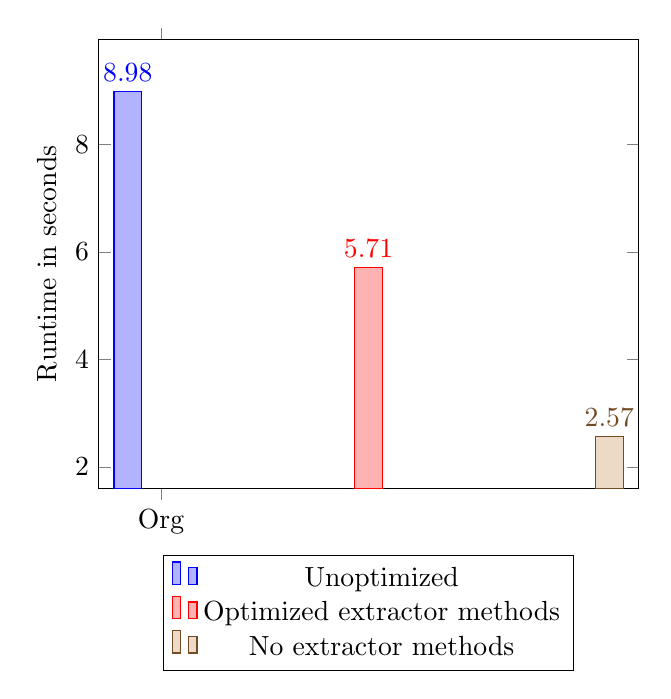
\begin{tikzpicture}
\begin{axis}[
    ybar,
    enlargelimits=0.15,
    legend style={at={(0.5,-0.15)},
      anchor=north,legend columns=1},
    ylabel={Runtime in seconds},
    symbolic x coords={Org, Opt1, Opt2},
    xtick=data,
    nodes near coords,
    nodes near coords align={vertical},
    ]
\addplot coordinates {(Org,8.98)};
\addplot coordinates {(Opt1,5.71)};
\addplot coordinates {(Opt2,2.57)};
\legend{Unoptimized ,Optimized extractor methods,No extractor methods}
\end{axis}
\end{tikzpicture}
\par{Using the original implementation as a baseline, we see that optimizing the extractor methods gives us a speed up of $1.57$, and if we get rid of the extractor methods all together we see a speedup of $3.49$}
\par{If we let the benchmarking program iterate over the list $2.5$ (up from 2), we see more drastic speedups as the unoptimized implementation runs out of memory}

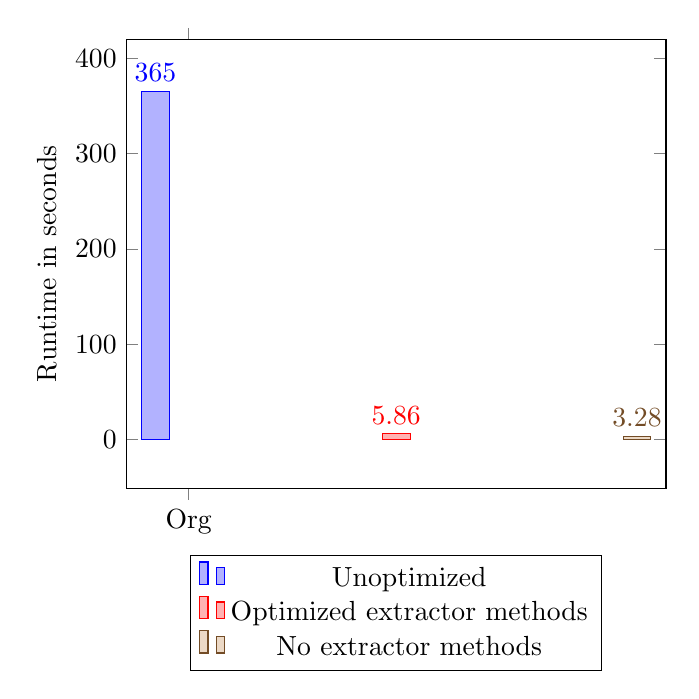
\begin{tikzpicture}
\begin{axis}[
    ybar,
    enlargelimits=0.15,
    legend style={at={(0.5,-0.15)},
      anchor=north,legend columns=1},
    ylabel={Runtime in seconds},
    symbolic x coords={Org, Opt1, Opt2},
    xtick=data,
    nodes near coords,
    nodes near coords align={vertical},
    ]
\addplot coordinates {(Org,365)};
\addplot coordinates {(Opt1,5.86)};
\addplot coordinates {(Opt2,3.28)};
\legend{Unoptimized ,Optimized extractor methods,No extractor methods}
\end{axis}
\end{tikzpicture}
\par{The speedup compared to the unoptimized versions here are far greater. For the implementation with optimized extractor methods the speedup is $62.28$ and the version without extractor methods is $111$ times faster. What this shows is that the original implementation for pattern matching is not only slow, but that it uses so much memory that it is impossible to use in a program that makes heavy use of ADTs to organize its data.}

\chapter{Conclusion and Future work}
\par{The goal of this thesis was to design and implement Algebraic Data Types in Encore, and also to optimize pattern matching. On both accounts I think it has been done successfully. The examples throughout this thesis shows how ADTs can make programs more compact, easier to read and increase programmer happiness\cite{happy}. The optimizations done to the pattern matching construct have also proven to be efficient, especially when it comes to space complexity. Without these improvements I doubt it would be feasible to add Algebraic Data Types to the Encore language.}
\par{However, we have throughout this thesis discussed some flaws with the implementation of ADTs. One such flaw is mentioned in section~\ref{ch:behaviour}. If a data constructor defines a method, it is not possible to ever call this method as the constructor method does not return an object of the correct type. To solve this some more syntactic sugar could be added to the pattern matching construct. If some variable \code{x} is matched to be of type \code{Foo}, then \code{x} could be typecasted to \code{Foo} so that we are able to call the method.}
%TODO: write about features I want to add, like binding a part as an object to an identifier
%#Källor:
%http://www.cs.cmu.edu/~rwh/pfpl.html
%\printbibliography

\chapter{References}


\begin{thebibliography}{9}
\bibitem{gustavL}
Gustav Lundin
\textit{Pattern Matching in Encore}.
http://www.diva-portal.org/smash/get/diva2:930151/FULLTEXT01.pdf

\bibitem{eBNF}
Wikipedia
\textit{Extended BNF}
https://en.wikipedia.org/wiki/Extended\_Backus\%E2\%80\%93Naur\_form

\bibitem{ABS}
Einar Broch JohnsenReiner HähnleJan SchäferRudolf SchlatteMartin Steffen
\textit{ABS: A Core Language for Abstract Behavioral Specification}
https://link.springer.com/chapter/10.1007\%2F978-3-642-25271-6\_8

\bibitem{ABSmut}
\textit{Algebraic Data Types in ABS}
http://abs-models.org/documentation/manual/\#sec:algebraic-data-types

\bibitem{ScalaCase}
\textit{Case classes in Scala}
https://docs.scala-lang.org/tour/case-classes.html

\bibitem{Encore}
Stephan Brandauer Elias Castegren Dave Clarke Kiko Fernandez-Reyes Einar Broch JohnsenKa I. PunS. Lizeth Tapia Tarifa Tobias Wrigstad Albert Mingkun Yang
\textit{Parallel Objects for Multicores: A Glimpse at the Parallel Language Encore}


\bibitem{happy}
Yukihiro Matsumoto on programmer happiness
\textit{https://maori.geek.nz/what-is-ruby-it-is-fun-and-makes-you-happy-337b6f10fa40}


%\bibitem{}
%http://haskell.cs.yale.edu/wp-content/uploads/2011/02/history.pdf
\end{thebibliography}


\begin{appendices}
\end{appendices}
\end{document}
